\documentclass[11pt]{article}
\usepackage[margin=1in]{geometry}
\usepackage{booktabs}
\usepackage{longtable}
\usepackage{array}
\usepackage{amsmath}
\usepackage{graphicx}
\usepackage[section]{placeins}
\usepackage{hyperref}
\hypersetup{colorlinks=true, linkcolor=blue, urlcolor=blue}
\sloppy
\newcolumntype{L}[1]{>{\raggedright\arraybackslash}p{#1}}

% Every number in this document is defined by build_exaction_panel.py (`report') in the
% generated files under tables/: \ex... for the measurements, \cl{<claim_id>} for the value
% of a verified legal claim. Nothing is typed by hand. The tables are one file, and
% \extable{<label>} places each where the text needs it.
% GENERATED BY build_exaction_panel.py report --- do not edit by hand.
\newcommand{\exAffordable}{188}
\newcommand{\exAlterations}{4{,}039}
\newcommand{\exAssumedGfa}{74}
\newcommand{\exBig}{843}
\newcommand{\exBigLinked}{380}
\newcommand{\exBunchEscPost}{942}
\newcommand{\exBunchEscPre}{880}
\newcommand{\exBunchEscRatio}{0.93}
\newcommand{\exBunchNoPost}{826}
\newcommand{\exBunchNoPre}{798}
\newcommand{\exBunchNoRatio}{0.97}
\newcommand{\exBunchTenPost}{70}
\newcommand{\exBunchTenPre}{83}
\newcommand{\exBunchTenRatio}{1.19}
\newcommand{\exBunchWeeks}{12}
\newcommand{\exClaims}{394}
\newcommand{\exClaimsUsed}{65}
\newcommand{\exClaimsVerified}{394}
\newcommand{\exCrossAgree}{53}
\newcommand{\exCrossAgreeTwo}{57}
\newcommand{\exCrossGf}{35}
\newcommand{\exCrossGfN}{17}
\newcommand{\exCrossLapsed}{46}
\newcommand{\exCrossLapsedN}{13}
\newcommand{\exCrossN}{121}
\newcommand{\exCrossNtwo}{107}
\newcommand{\exCrossRows}{260}
\newcommand{\exCrossSeventeen}{50}
\newcommand{\exCrossSeventeenN}{30}
\newcommand{\exCrossSix}{84}
\newcommand{\exCrossSixN}{19}
\newcommand{\exCrossThirteen}{52}
\newcommand{\exCrossThirteenN}{23}
\newcommand{\exCrossTwo}{69}
\newcommand{\exCrossTwoN}{13}
\newcommand{\exCutPost}{221}
\newcommand{\exCutPre}{214}
\newcommand{\exDbiApp}{26}
\newcommand{\exDensity}{49}
\newcommand{\exDensityBig}{45}
\newcommand{\exEffSix}{2006-09-09}
\newcommand{\exEffSixInferred}{2006-09-09}
\newcommand{\exElevenA}{3}
\newcommand{\exFiveSix}{4}
\newcommand{\exFourSix}{14}
\newcommand{\exGpu}{841}
\newcommand{\exGpuHi}{1{,}086}
\newcommand{\exGpuLo}{645}
\newcommand{\exGpuN}{1{,}284}
\newcommand{\exInclShare}{81}
\newcommand{\exLegalClaims}{112}
\newcommand{\exLinked}{966}
\newcommand{\exMedLag}{1.7}
\newcommand{\exNA}{131}
\newcommand{\exNB}{145}
\newcommand{\exNC}{99}
\newcommand{\exND}{25}
\newcommand{\exNineA}{18}
\newcommand{\exNineSix}{6}
\newcommand{\exPaySentenceAbsent}{2026}
\newcommand{\exPaySentenceFirst}{2011}
\newcommand{\exPaySentenceLast}{2025}
\newcommand{\exPipe}{94}
\newcommand{\exPriced}{400}
\newcommand{\exPricedLinked}{254}
\newcommand{\exProjects}{3{,}574}
\newcommand{\exPuHi}{\$78k}
\newcommand{\exPuLo}{\$50k}
\newcommand{\exPuMed}{\$61k}
\newcommand{\exPuMedA}{\$52k}
\newcommand{\exPuMedB}{\$71k}
\newcommand{\exPuMedC}{\$66k}
\newcommand{\exPuMedD}{\$64k}
\newcommand{\exPuMedLinked}{\$62k}
\newcommand{\exPuMedNot}{\$58k}
\newcommand{\exRegFirst}{2011}
\newcommand{\exRegLast}{2026}
\newcommand{\exRegisterClaims}{282}
\newcommand{\exRegisters}{15}
\newcommand{\exSbThreeThirty}{42}
\newcommand{\exShareHi}{28}
\newcommand{\exShareLo}{15}
\newcommand{\exShareMed}{20}
\newcommand{\exShareMedLinked}{21}
\newcommand{\exShareMedNot}{19}
\newcommand{\exStepTen}{\$420k}
\newcommand{\exStepTenPerUnit}{\$42k}
\newcommand{\exStepTsf}{\$209k}
\newcommand{\exStepTwentyFive}{\$525k}
\newcommand{\exStepTwentyFiveB}{\$26k}
\newcommand{\exStepYear}{2026}
\newcommand{\exTenA}{5}
\newcommand{\exTenSix}{2}
\newcommand{\exTenureGapMax}{\$20k}
\newcommand{\exTenureGapMed}{\$0k}
\newcommand{\exTfr}{124}
\newcommand{\exTwentyA}{4}
\newcommand{\exTwentyFiveA}{4}
\newcommand{\exTwentyFourA}{10}
\newcommand{\exTwentyOneA}{1}
\newcommand{\exUmu}{49}
\newcommand{\exVersions}{8}
\newcommand{\exWindow}{59}
\makeatletter
\expandafter\def\csname cl@inc2002_apply\endcsname{2001-06-18}
\expandafter\def\csname cl@inc2002_threshold\endcsname{10}
\expandafter\def\csname cl@inc2002_onsite_10\endcsname{10}
\expandafter\def\csname cl@inc2002_onsite_12\endcsname{12}
\expandafter\def\csname cl@inc2002_offsite_15\endcsname{15}
\expandafter\def\csname cl@inc2002_offsite_17\endcsname{17}
\expandafter\def\csname cl@inc2002_fee_basis\endcsname{off-site unit count x affordability gap}
\expandafter\def\csname cl@inc2002_transition\endcsname{5}
\expandafter\def\csname cl@inc2002_effective\endcsname{2002-04-05}
\expandafter\def\csname cl@inc2006_5to9\endcsname{2006-07-18}
\expandafter\def\csname cl@inc2006_onsite_15\endcsname{15}
\expandafter\def\csname cl@inc2006_offsite_20\endcsname{20}
\expandafter\def\csname cl@inc2006_vesting\endcsname{first site/building permit}
\expandafter\def\csname cl@inc2006_passed\endcsname{2006-08-01}
\expandafter\def\csname cl@inc2006_sep9\endcsname{2006-09-09}
\expandafter\def\csname cl@inc2006_enacted\endcsname{2006-08-10}
\expandafter\def\csname cl@inc2013_table_fee20\endcsname{20}
\expandafter\def\csname cl@inc2013_table_onsite12\endcsname{12}
\expandafter\def\csname cl@inc2013_table_offsite20\endcsname{20}
\expandafter\def\csname cl@inc2013_table_july18\endcsname{2006-07-18}
\expandafter\def\csname cl@inc2013_threshold10\endcsname{2013-01-15}
\expandafter\def\csname cl@inc2013_table_disclaimer\endcsname{yes}
\expandafter\def\csname cl@inc2013_effective\endcsname{2013-05-10}
\expandafter\def\csname cl@inc2016_fee20\endcsname{20}
\expandafter\def\csname cl@inc2016_fee33\endcsname{33}
\expandafter\def\csname cl@inc2016_onsite\endcsname{12 / 25}
\expandafter\def\csname cl@inc2016_fee_timing\endcsname{first construction document}
\expandafter\def\csname cl@propc2016\endcsname{2016-06-07}
\expandafter\def\csname cl@propc2016_contingent\endcsname{Charter 16.110}
\expandafter\def\csname cl@propc2012\endcsname{2012-11}
\expandafter\def\csname cl@ord_effective_30days\endcsname{30 days}
\expandafter\def\csname cl@inc2016_effective\endcsname{2016-06-12}
\expandafter\def\csname cl@inc2017_effective\endcsname{2017-08-26}
\expandafter\def\csname cl@inc2017_cutoff\endcsname{2016-01-12}
\expandafter\def\csname cl@inc2017_after2016\endcsname{2016-01-12}
\expandafter\def\csname cl@cod_4153_pre2016\endcsname{2016-01-12}
\expandafter\def\csname cl@cod_4153_25plus\endcsname{2013-01-01}
\expandafter\def\csname cl@cod_4153_on13\endcsname{13}
\expandafter\def\csname cl@cod_4153_on135\endcsname{13.5}
\expandafter\def\csname cl@cod_4153_on145\endcsname{14.5}
\expandafter\def\csname cl@cod_4153_fee25\endcsname{25}
\expandafter\def\csname cl@cod_4153_fee275\endcsname{27.5}
\expandafter\def\csname cl@cod_4153_fee30\endcsname{30}
\expandafter\def\csname cl@cod_4153_deadline\endcsname{2018-12-07}
\expandafter\def\csname cl@cod_4153_exempt\endcsname{2016-01-12}
\expandafter\def\csname cl@cod_4153_threshold\endcsname{10}
\expandafter\def\csname cl@cod_4155_fee20\endcsname{20}
\expandafter\def\csname cl@cod_4155_fee33\endcsname{33}
\expandafter\def\csname cl@cod_4155_fee30\endcsname{30}
\expandafter\def\csname cl@cod_4155_vesting\endcsname{complete EEA date}
\expandafter\def\csname cl@cod_4155_30months\endcsname{30 months}
\expandafter\def\csname cl@cod_4155_timing\endcsname{402(d)}
\expandafter\def\csname cl@cod_4155_dbl\endcsname{yes}
\expandafter\def\csname cl@cod_4156_on12\endcsname{12}
\expandafter\def\csname cl@cod_4156_on20\endcsname{20}
\expandafter\def\csname cl@cod_4156_on18\endcsname{18}
\expandafter\def\csname cl@cod_4156_esc_small\endcsname{0.5}
\expandafter\def\csname cl@cod_4156_esc_large1\endcsname{1.0}
\expandafter\def\csname cl@cod_4156_esc_large2\endcsname{0.5}
\expandafter\def\csname cl@cod_4156_caps\endcsname{26 / 24}
\expandafter\def\csname cl@cod_4156_vesting\endcsname{complete EEA date}
\expandafter\def\csname cl@cod_4156b_same\endcsname{20 / 18}
\expandafter\def\csname cl@inc2023_effective\endcsname{2023-11-12}
\expandafter\def\csname cl@a415_pipeline\endcsname{2023-11-01}
\expandafter\def\csname cl@a415_final_approval\endcsname{first development application}
\expandafter\def\csname cl@a415_request\endcsname{2026-11-01}
\expandafter\def\csname cl@a415_fee164\endcsname{16.4}
\expandafter\def\csname cl@a415_onsite12_small\endcsname{12}
\expandafter\def\csname cl@a415_onsite12_large\endcsname{12}
\expandafter\def\csname cl@a415_offsite164\endcsname{16.4}
\expandafter\def\csname cl@b415_window\endcsname{2023-11-01 to 2026-11-01}
\expandafter\def\csname cl@b415_fee205\endcsname{20.5}
\expandafter\def\csname cl@b415_onsite15\endcsname{15}
\expandafter\def\csname cl@area_specific_rates\endcsname{area-specific}
\expandafter\def\csname cl@b415_sunset\endcsname{2026-11-01}
\expandafter\def\csname cl@o201_operative\endcsname{2026-11-21}
\expandafter\def\csname cl@o201_2026_fee27\endcsname{27}
\expandafter\def\csname cl@o201_2026_fee245\endcsname{24.5}
\expandafter\def\csname cl@o201_2026_onsite15\endcsname{15}
\expandafter\def\csname cl@o201_2026_fee20\endcsname{20}
\expandafter\def\csname cl@o201_2026_on20o\endcsname{20}
\expandafter\def\csname cl@o201_2026_on18r\endcsname{18}
\expandafter\def\csname cl@o201_2026_off27o\endcsname{27}
\expandafter\def\csname cl@o201_2026_esc\endcsname{2028-01-01}
\expandafter\def\csname cl@fee_402d_timing\endcsname{first construction document}
\expandafter\def\csname cl@fee_409_index\endcsname{January 1}
\expandafter\def\csname cl@fee_rate_at_payment\endcsname{payment date}
\expandafter\def\csname cl@fee_193_approval\endcsname{final approval}
\expandafter\def\csname cl@fee_193_effective\endcsname{2023-10-16}
\expandafter\def\csname cl@fee_tfr33\endcsname{33}
\expandafter\def\csname cl@fee_tfr_tsf\endcsname{411A}
\expandafter\def\csname cl@tsf_threshold\endcsname{21}
\expandafter\def\csname cl@tsf_base\endcsname{7.74 / 8.74}
\expandafter\def\csname cl@tsf_created\endcsname{2015-12-25}
\expandafter\def\csname cl@cc_threshold\endcsname{1}
\expandafter\def\csname cl@cc_created\endcsname{2016-02-18}
\expandafter\def\csname cl@cc_base\endcsname{1.83 / 0.91}
\expandafter\def\csname cl@jhl_nonres\endcsname{non-residential}
\expandafter\def\csname cl@area_en_start\endcsname{2008-12-19}
\expandafter\def\csname cl@area_mo421_start\endcsname{2008-04-03}
\expandafter\def\csname cl@area_mo416_start\endcsname{2008-05-30}
\expandafter\def\csname cl@area_rh_start\endcsname{2005-08-19}
\expandafter\def\csname cl@area_soma_start\endcsname{2005-08-19}
\expandafter\def\csname cl@area_vv_start\endcsname{2005-11-18}
\expandafter\def\csname cl@area_bp_start\endcsname{2009-04-17}
\expandafter\def\csname cl@area_tc_start\endcsname{2012-09-07}
\expandafter\def\csname cl@area_cs_start\endcsname{2019-01-12}
\expandafter\def\csname cl@sb330_freeze\endcsname{preliminary application}
\expandafter\def\csname cl@sb330_index_exception\endcsname{cost index}
\expandafter\def\csname cl@sb330_chapter\endcsname{Stats. 2019, ch. 654}
\expandafter\def\csname cl@sb330_approved\endcsname{2019-10-09}
\expandafter\def\csname cl@gov_standards_fees\endcsname{yes}
\makeatother
\newcommand{\cl}[1]{\csname cl@#1\endcsname}

\newcommand{\extable}[1]{\FloatBarrier\def\extab{#1}% GENERATED BY build_exaction_panel.py report --- do not edit by hand.
\ifnum\pdfstrcmp{\extab}{excoverage}=0
\begin{table}[htbp]\centering\small
\caption{Coverage: what each project's dates, floor area and tenure come from, and how many are priced. New construction (DBI permit types 1 and 2) adding at least one unit, one row per project (a Commission case collapsed to its principal permit).}\label{tab:excoverage}
\begin{tabular}{L{10.2cm}rr}\toprule & All & 10+ units\\\midrule
Residential new-construction projects filed since 2001-06-18 & 3{,}574 & 843\\
\quad of which Commission-linked (T1/T2) & 966 & 380\\
Application date from a planning record & 2{,}629 & 671\\
Application date = the DBI filing (no planning record found) & 945 & 172\\
Approval = a Commission action & 799 & 312\\
Approval = DBI approval or issuance & 2{,}003 & 385\\
Not yet approved (held to the version in force) & 772 & 146\\
First construction document recorded by DBI & 1{,}816 & 490\\
\quad issuance used in its place & 769 & 127\\
Floor area from a PRJ record & 919 & 395\\
Floor area assumed (units x median) & 2{,}655 & 448\\
Tenure known (MOHCD pipeline) & 63 & 62\\
Tenure from description words only & 171 & 82\\
100\% affordable (outside the program) & 188 & 161\\
Density bonus mentioned (state or HOME-SF) & 49 & 45\\
Obligation marked uncertain (density bonus, UMU or SB 330) & 118 & 88\\
SB 330 preliminary application flagged & 42 & 24\\
In a UMU district (Section 419 replaces the citywide rates) & 49 & 39\\
Eligible for the 2023 pipeline relief (415A) & 94 & 94\\
Under the 2023--26 window (415B) & 59 & 59\\
Impact fees cut 33\% (201-23's temporary reduction) & 124 & 27\\
Rate year 2017 (no register: interpolated) & 178 & 39\\
Priced in full (inclusionary and every impact fee) & 1{,}723 & 498\\
\bottomrule\end{tabular}\end{table}
\fi
\ifnum\pdfstrcmp{\extab}{exversions}=0
\begin{table}[htbp]\centering\small
\caption{The inclusionary versions, as the enacted ordinances state them. Shares are percent of the project's units; R rental, O ownership; a slash separates the 10--24 and 25+ unit tiers. Every figure is a verified claim in \texttt{exaction\_sources.csv} (Section~\ref{sec:exsources}).}\label{tab:exversions}
\resizebox{\textwidth}{!}{\begin{tabular}{llL{2.1cm}L{5.4cm}L{2.9cm}L{2.2cm}L{2.2cm}l}\toprule
Version & Source & In force from & Which projects & On-site & Fee & Off-site & Units\\\midrule
2002 & Ord.\ 37-02 & 2002-04-05 & first application from 2001-06-18 & 10 (12 CU/PUD) & 15 (17) & = off-site & 10+\\
2006 & Ords.\ 213-06, 219-06 & 2006-09-09 & first application from 2006-07-18 & 15 & 20 & 20 & 5+\\
2013 & Ord.\ 62-13 & 2013-05-10 & same; 5--9 units out without a first construction document by 2013-01-15 & 12 & 20 & 20 & 10+\\
2016 & Prop.\ C; Ord.\ 76-16 & 2016-06-12 & complete EEA; EEA 2013--2016-01-12 grandfathered (25+: 13/13.5/14.5 on-site, 25/27.5/30 fee) if approved by 2018-12-07 & 12 / 25 & 20 / 33 & 20 / 33 & 10--24 / 25+\\
2017 & Ord.\ 158-17 & 2017-08-26 & complete EEA after 2016-01-12; on-site share rises each January 1 by EEA year & 12$\to$15 / 18$\to$24 R, 20$\to$26 O & 20 / 30 R, 33 O & 20 / 30 R, 33 O & 10--24 / 25+\\
2023 pipeline & Ord.\ 201-23, 415A & 2023-11-12 & approved before 2023-11-01, no first construction document; on request by 2026-11-01 & 12 & 16.4 & 16.4 & 10+\\
2023 window & Ord.\ 201-23, 415B & 2023-11-12 & approved 2023-11-01 to 2026-11-01, first construction document within 30 months & 15 (25+) & 20.5 (25+) & 20.5 (25+) & 25+\\
2026 & Ord.\ 201-23, s.\ 7 & 2026-11-21 & operative 2026-11-21 unless amended & 15 / 20 O & 20 / 24.5 R, 27 O & --- & 10--24 / 25+\\
\bottomrule\end{tabular}}\end{table}
\fi
\ifnum\pdfstrcmp{\extab}{exregisters}=0
\begin{table}[htbp]\centering\scriptsize
\caption{Residential rates by register year, dollars per gross square foot except the inclusionary affordability gap (dollars per unit, used until the 2019 register). Each cell is a verified claim quoting the register. No 2017 register was found.}\label{tab:exregisters}
\resizebox{\textwidth}{!}{\begin{tabular}{lrrrrrrrrrrrrrrr}\toprule
Rate & 2011 & 2012 & 2013 & 2014 & 2015 & 2016 & 2018 & 2019 & 2020 & 2021 & 2022 & 2023 & 2024 & 2025 & 2026\\\midrule
Inclusionary, per 1-bedroom (gap) & 248{,}210 & 248{,}210 & 236{,}545 & 261{,}271 & 270{,}441 & 268{,}960 & 268{,}960 &  &  &  &  &  &  &  & \\
Inclusionary, per gsf &  &  &  &  &  &  &  & 199.50 & 210.47 & 217.84 & 230.91 & 244.76 & 249.66 & 249.66 & 249.66\\
TSF, 21--99 units &  &  &  &  &  & 7.74 & 8.60 & 9.11 & 9.61 & 9.95 & 10.55 & 11.18 & 11.40 & 11.63 & 11.86\\
TSF, 100+ units &  &  &  &  &  & 8.74 & 9.71 & 10.29 & 10.86 & 11.24 & 11.91 & 12.62 & 12.87 & 13.13 & 13.39\\
Child care, 10+ units &  &  &  &  &  & 1.83 & 2.03 & 2.15 & 2.27 & 2.35 & 2.49 & 2.64 & 2.69 & 2.74 & 2.80\\
Child care, 1--9 units &  &  &  &  &  & 0.91 & 1.02 & 1.08 & 1.14 & 1.18 & 1.25 & 1.33 & 1.36 & 1.39 & 1.41\\
School (SFUSD) & 2.24 & 2.24 & 2.24 & 2.91 & 2.91 & 3.36 & 3.48 & 3.79 & 3.79 & 3.79 & 3.79 & 3.79 & 3.79 & 3.79 & 3.79\\
Eastern Neighborhoods, Tier 1 & 8.24 & 8.51 & 8.85 & 9.25 & 9.71 & 10.19 & 11.32 & 12.00 & 12.66 & 13.10 & 13.89 & 14.72 & 15.01 & 15.31 & 15.62\\
Eastern Neighborhoods, Tier 3 & 16.48 & 17.02 & 17.70 & 18.49 & 19.42 & 20.39 & 22.64 & 24.00 & 25.32 & 26.21 & 27.78 & 29.45 & 30.04 & 30.64 & 31.24\\
Market \& Octavia (421) & 9.27 & 9.57 & 9.95 & 10.40 & 10.92 & 11.47 & 12.73 & 13.49 & 14.23 & 14.73 & 15.61 & 16.55 & 16.88 & 17.22 & 17.57\\
Market \& Octavia affordable (416, NCT) & 3.71 & 3.83 & 3.98 & 4.16 & 4.37 & 4.59 & 5.10 & 5.40 & 5.70 & 5.90 & 6.25 & 6.63 & 6.76 & 6.90 & 7.03\\
Rincon Hill & 8.86 & 9.15 & 9.51 & 9.94 & 10.44 & 10.96 & 12.17 & 12.90 & 13.61 & 14.09 & 14.94 & 15.84 & 16.16 & 16.48 & 16.79\\
SOMA stabilization & 11.28 & 11.65 & 12.11 & 12.66 & 13.29 & 13.95 & 15.49 & 16.42 & 17.32 & 17.93 & 19.01 & 20.15 & 20.55 & 20.96 & 21.38\\
Visitacion Valley & 4.72 & 4.87 & 5.07 & 5.29 & 5.56 & 5.84 & 6.48 & 6.87 & 7.25 & 7.50 & 7.95 & 8.43 & 8.60 & 8.77 & 8.94\\
Balboa Park & 8.24 & 8.51 & 8.85 & 9.25 & 9.71 & 10.19 & 11.32 & 12.00 & 12.66 & 13.10 & 13.89 & 14.72 & 15.01 & 15.31 & 15.62\\
Central SoMa 433, Tier B condo &  &  &  &  &  &  &  & 20.00 & 21.10 & 21.84 & 23.15 & 24.54 & 25.03 & 25.53 & 26.04\\
\bottomrule\end{tabular}}\end{table}
\fi
\ifnum\pdfstrcmp{\extab}{exvesting}=0
\begin{table}[htbp]\centering\small
\caption{When each part of the obligation is fixed, and the claim that says so.}\label{tab:exvesting}
\begin{tabular}{L{3.6cm}L{8.2cm}L{3.4cm}}\toprule Component & Fixed at & Claims\\\midrule
Inclusionary share (\%) & the first application (2002--2013; 62-13's Table 415.3); the complete EEA from 2016, with the on-site escalation read at the EEA date; approval-date windows in 2016--18 (grandfathering deadline) and 2023--26 (415A, 415B); lapses without a site or building permit within 30 months of approval & \scriptsize inc2013\_table\_july18, cod\_4155\_vesting, cod\_4156\_vesting, cod\_4153\_deadline, cod\_4155\_30months\\
Inclusionary fee (\$) & the share x MOHCD's rate at payment, due at the first construction document; the fee is outside 193-23's approval-date freeze & \scriptsize cod\_4155\_timing, inc2016\_fee\_timing, fee\_193\_approval\\
Impact fees (types and \$) & before 2023-10-16: the rate in force when paid, whatever the filing date; from 2023-10-16: the types and rates in force at Final Approval & \scriptsize fee\_rate\_at\_payment, fee\_402d\_timing, fee\_193\_approval, fee\_193\_effective\\
Everything, for a housing project with an SB 330 preliminary application (2020--) & the ordinances, policies and standards in force at the complete preliminary application, fees included, except automatic index adjustments & \scriptsize sb330\_freeze, gov\_standards\_fees, sb330\_index\_exception\\
\bottomrule\end{tabular}\end{table}
\fi
\ifnum\pdfstrcmp{\extab}{exobligation}=0
\begin{table}[htbp]\centering\small
\caption{The priced obligation of new buildings of 10 or more units, per unit and as a share of DBI's valuation, by the year the impact fees vested. Lower bound: rental rates where tenure matters; upper: ownership. Quantiles across projects.}\label{tab:exobligation}
\begin{tabular}{llrrrrrrr}\toprule
Vested & Group & $n$ & \multicolumn{3}{c}{\$ per unit (lower bound)} & \multicolumn{3}{c}{Share of valuation (\%)}\\\cmidrule(lr){4-6}\cmidrule(lr){7-9} & & & p25 & median & p75 & p25 & median & p75\\\midrule
2011--15 & all & 131 & \$45k & \$52k & \$57k & 14 & 18 & 25\\
 & Commission-linked & 87 & \$45k & \$52k & \$57k & 14 & 18 & 25\\
 & not linked & 44 & \$48k & \$52k & \$57k & 14 & 18 & 23\\
2016--19 & all & 145 & \$63k & \$71k & \$91k & 18 & 23 & 30\\
 & Commission-linked & 92 & \$63k & \$72k & \$91k & 18 & 23 & 30\\
 & not linked & 53 & \$63k & \$69k & \$88k & 19 & 23 & 28\\
2020--23 & all & 99 & \$49k & \$66k & \$88k & 14 & 20 & 27\\
 & Commission-linked & 60 & \$52k & \$76k & \$104k & 17 & 22 & 29\\
 & not linked & 39 & \$46k & \$60k & \$70k & 11 & 17 & 22\\
2024--26 & all & 25 & \$53k & \$64k & \$88k & 13 & 19 & 26\\
 & Commission-linked & 15 & \$57k & \$80k & \$93k & 16 & 23 & 34\\
 & not linked & 10 & \$53k & \$54k & \$61k & 10 & 14 & 18\\
\bottomrule\end{tabular}\end{table}
\fi
\ifnum\pdfstrcmp{\extab}{excross}=0
\begin{table}[htbp]\centering\small
\caption{The schedule against the Commission's own conditions: cases whose conditions print an inclusionary percentage (\texttt{conditions\_numeric.parquet}), and whether that percentage equals one the schedule assigns the case (on-site, fee or off-site, either tenure, or the 415A option). A case agrees if any of its printed percentages does.}\label{tab:excross}
\begin{tabular}{lrrr}\toprule Version assigned & Cases & Agree & \%\\\midrule
100\% affordable (outside the program) & 3 & 0 & 0\\
2002 (Ord. 37-02) & 13 & 9 & 69\\
2006 (Ords. 213-06, 219-06) & 19 & 16 & 84\\
2013 (Ord. 62-13) & 23 & 12 & 52\\
2016 grandfathered tiers (Ord. 76-16, 415.3(b)) & 17 & 6 & 35\\
2017 (Ord. 158-17) & 30 & 15 & 50\\
2017 (Ord. 158-17), grandfathering lapsed & 13 & 6 & 46\\
2023 window (Ord. 201-23, 415B) & 3 & 0 & 0\\
\midrule All & 121 & 64 & 53\\
Outside UMU, not 100\% affordable & 107 & 61 & 57\\
\bottomrule\end{tabular}\end{table}
\fi
\ifnum\pdfstrcmp{\extab}{exnotch}=0
\begin{table}[htbp]\centering\small
\caption{New buildings by unit count around the thresholds, by filing period (100\% affordable projects excluded). The inclusionary threshold is 10 units except 2006--2013, when it was 5; from 2016 a second tier begins at 25; the TSF begins above 20.}\label{tab:exnotch}
\resizebox{\textwidth}{!}{\begin{tabular}{lrrrrrrrrrrrrrrr}\toprule
Filed & 4 & 5 & 6 & 8 & 9 & 10 & 11 & 19 & 20 & 21 & 22 & 23 & 24 & 25 & 26\\\midrule
threshold 10 (37-02) & 28 & 11 & 31 & 22 & 8 & 4 & 2 & 3 & 6 & 5 & 2 & 1 & 3 & 1 & 6\\
threshold 5 (213-06) & 14 & 4 & 8 & 6 & 6 & 2 & 2 & 2 & 2 & 3 & 0 & 2 & 1 & 2 & 0\\
threshold 10 (62-13) & 13 & 5 & 8 & 3 & 13 & 1 & 8 & 2 & 6 & 4 & 1 & 2 & 3 & 0 & 0\\
threshold 10; 25+ tier (76-16, 158-17) & 42 & 22 & 15 & 16 & 18 & 5 & 3 & 2 & 4 & 1 & 3 & 0 & 10 & 4 & 0\\
\bottomrule\end{tabular}}\end{table}
\fi
\ifnum\pdfstrcmp{\extab}{exclaims}=0
{\scriptsize\begin{longtable}{L{3.0cm}L{4.6cm}L{2.0cm}L{4.6cm}}
\caption{Every legal claim the schedule reads, with its value and the first words of its quotation. The register rates (282 further claims) are in \texttt{exaction\_sources.csv}.}\label{tab:exclaims}\\\toprule
Claim & Field & Value & Quotation (start)\\\midrule\endfirsthead\toprule Claim & Field & Value & Quotation (start)\\\midrule\endhead
inc2002\_\allowbreak{}apply & applies to applications filed on or after & 2001-06-18 & \textit{on or after June 18, 2001 for housing projects which}\\
inc2002\_\allowbreak{}threshold & unit threshold & 10 & \textit{consist often or more units; and do not require}\\
inc2002\_\allowbreak{}onsite\_\allowbreak{}10 & on-site share, no CU/PUD & 10 & \textit{315.3(a)(1), as a condition ofPlanning Department approval ofa project's building pennit, that 10\%}\\
inc2002\_\allowbreak{}onsite\_\allowbreak{}12 & on-site share, CU/PUD/live-work & 12 & \textit{live/work project that 12 12\% ofall units constructed on the project site}\\
inc2002\_\allowbreak{}offsite\_\allowbreak{}15 & off-site share, no CU/PUD & 15 & \textit{For projects described in 315.3(a)(1), 15\% as follows}\\
inc2002\_\allowbreak{}offsite\_\allowbreak{}17 & off-site share, CU/PUD/live-work & 17 & \textit{For projects described in 315.3(a)(2),(3), and (4),170/0 as follows}\\
inc2002\_\allowbreak{}fee\_\allowbreak{}basis & in-lieu fee basis & off-site unit count x affordability gap & \textit{The number ofunits required bv Section 315.5 ifthe project applicant were to elect to 8 meet the requiremen...}\\
inc2002\_\allowbreak{}transition & transitional on-site share, first 180 days, no CU/PUD & 5 & \textit{from the effective date ofthis legislation and 180 days thereafter shall be 5\%}\\
inc2002\_\allowbreak{}effective & program effective date & 2002-04-05 & \textit{(b) The effective date of these requirements shall be either April 5, 2002, which is the}\\
inc2006\_\allowbreak{}5to9 & threshold lowered to 5 units for first applications on or after & 2006-07-18 & \textit{first application, including an environmental evaluation application or any other Planning 17 Department ap...}\\
inc2006\_\allowbreak{}onsite\_\allowbreak{}15 & on-site share, all project types & 15 & \textit{applicant must constructzc ./5 times the total number}\\
inc2006\_\allowbreak{}offsite\_\allowbreak{}20 & off-site share & 20 & \textit{H\% 20\% so that a project applicant must construct}\\
inc2006\_\allowbreak{}vesting & vesting: first site or building permit before the effective date keeps prior requirements & first site/building permit & \textit{projects that have received a first site or building permit prior to the effective date of this 3 legislati...}\\
inc2006\_\allowbreak{}passed & Ord. 219-06 finally passed & 2006-08-01 & \textit{FINALLY PASSED on August 1,2006}\\
inc2006\_\allowbreak{}sep9 & the 2006 amendments operative from & 2006-09-09 & \textit{approval on or after September 9, compliance option 2006}\\
inc2006\_\allowbreak{}enacted & Ord. 219-06 passed date in Legistar & 2006-08-10 & \textit{"MatterPassedDate":\allowbreak{}"2006-08-10T00:\allowbreak{}00:\allowbreak{}00"}\\
inc2013\_\allowbreak{}table\_\allowbreak{}fee20 & fee share, first application on or after 2006-07-18 & 20 & \textit{20\% Fee}\\
inc2013\_\allowbreak{}table\_\allowbreak{}onsite12 & on-site share, first application on or after 2006-07-18 (as of 62-13) & 12 & \textit{12\% on-site*}\\
inc2013\_\allowbreak{}table\_\allowbreak{}offsite20 & off-site share, first application on or after 2006-07-18 & 20 & \textit{20\% off-site*}\\
inc2013\_\allowbreak{}table\_\allowbreak{}july18 & date column of the percentages row & 2006-07-18 & \textit{application on or after July 18, 2006 .J..§.12\% on-site*}\\
inc2013\_\allowbreak{}threshold10 & threshold back to 10: 5-9 unit projects without a first construction document by & 2013-01-15 & \textit{construction document as of January 15,2013}\\
inc2013\_\allowbreak{}table\_\allowbreak{}disclaimer & the ordinances prevail over the table & yes & \textit{the 23 implementing ordinances shall prevail}\\
inc2013\_\allowbreak{}effective & Ord. 62-13 effective & 2013-05-10 & \textit{121162 0062-13 05/10/2013 Planning Code - Inclusionary Affordable Housing Program, Updates, and Clarificati...}\\
inc2016\_\allowbreak{}fee20 & fee share, 10-24 units & 20 & \textit{The applicable percentage shall be 20\% percent [or 19 housing development projects consisting of 10 dwellin...}\\
inc2016\_\allowbreak{}fee33 & fee share, 25+ units & 33 & \textit{consisting of 25 dwelling units or more shall be 21 33\%}\\
inc2016\_\allowbreak{}onsite & on-site share, 10-24 / 25+ units & 12 / 25 & \textit{that 12\% or 25\% percent, as applicable}\\
inc2016\_\allowbreak{}fee\_\allowbreak{}timing & fee due at first construction document & first construction document & \textit{at the time of and in no 1 O event later than issuance of the first construction document}\\
propc2016 & Proposition C (Charter 16.110) approved by the voters & 2016-06-07 & \textit{following voter approval of Proposition Cat the June 7, 2016 election to revise the 13 City Charter's inclu...}\\
propc2016\_\allowbreak{}contingent & 76-16's new percentages effective only with the June 2016 Charter amendment & Charter 16.110 & \textit{will become effective only on the effective date of the 16 Charter amendment revising Section 16.110 at the...}\\
propc2012 & Proposition C (November 2012) codified in part as Charter 16.110 & 2012-11 & \textit{In ~V-ovember 2012 the voters amended the Charter by adopting Pr0J3osition C}\\
ord\_\allowbreak{}effective\_\allowbreak{}30days & SF ordinances take effect 30 days after enactment & 30 days & \textit{This ordinance shall become effective 30 days after 16 enactment}\\
inc2016\_\allowbreak{}effective & Ord. 76-16 effective & 2016-06-12 & \textit{160255 0076-16 06/12/2016 Planning, Administrative Codes - Inclusionary Affordable Housing Fee and Requirem...}\\
inc2017\_\allowbreak{}effective & Ord. 158-17 effective & 2017-08-26 & \textit{161351 0158-17 08/26/2017 Planning Code - Inclusionary Affordable Housing Fee and Dwelling Unit Mix Require...}\\
inc2017\_\allowbreak{}cutoff & the keep-prior-requirements cutoff moved from 2013-01-01 to 2016-01-12 & 2016-01-12 & \textit{application prior to January 4, ~ 12, 2016 shall comply with the Affordable Housing Fee}\\
inc2017\_\allowbreak{}after2016 & EEA after 2016-01-12: Sections 415.5-415.7 as applicable & 2016-01-12 & \textit{Any development project that submits an Environmental Evaluation 18 application after January 12, 2016, sha...}\\
cod\_\allowbreak{}4153\_\allowbreak{}pre2016 & complete EEA before 2016-01-12 keeps the requirements in effect on 2016-01-12 & 2016-01-12 & \textit{any development project that has submitted a complete Environmental Evaluation application prior to January...}\\
cod\_\allowbreak{}4153\_\allowbreak{}25plus & grandfathering tiers apply to projects of 25+ units with EEA on or after 2013-01-01 & 2013-01-01 & \textit{For development projects that have submitted a complete Environmental Evaluation application on or after Ja...}\\
cod\_\allowbreak{}4153\_\allowbreak{}on13 & on-site, 25+, EEA before 2014-01-01 & 13 & \textit{prior to January 1, 2014 shall provide affordable units in the amount of 13\% of the number of units constru...}\\
cod\_\allowbreak{}4153\_\allowbreak{}on135 & on-site, 25+, EEA before 2015-01-01 & 13.5 & \textit{prior to January 1, 2015 shall provide affordable units in the amount of 13.5\% of the number of units const...}\\
cod\_\allowbreak{}4153\_\allowbreak{}on145 & on-site, 25+, EEA on or before 2016-01-12 & 14.5 & \textit{on or prior to January 12, 2016 shall provide affordable units in the amount of 14.5\% of the number of unit...}\\
cod\_\allowbreak{}4153\_\allowbreak{}fee25 & fee/off-site, 25+, EEA before 2014-01-01 & 25 & \textit{prior to January 1, 2014, shall pay a fee or provide off-site housing in an amount equivalent to 25\% of the...}\\
cod\_\allowbreak{}4153\_\allowbreak{}fee275 & fee/off-site, 25+, EEA before 2015-01-01 & 27.5 & \textit{prior to January 1, 2015, shall pay a fee or provide off-site housing in an amount equivalent to 27.5\% of t...}\\
cod\_\allowbreak{}4153\_\allowbreak{}fee30 & fee/off-site, 25+, EEA on or before 2016-01-12 & 30 & \textit{on or prior to January 12, 2016 shall pay a fee or provide off-site housing in an amount equivalent to 30\% ...}\\
cod\_\allowbreak{}4153\_\allowbreak{}deadline & grandfathered tiers lapse if not approved on or before 2018-12-07 & 2018-12-07 & \textit{In the event the project has not been approved, which shall mean approval following any administrative appe...}\\
cod\_\allowbreak{}4153\_\allowbreak{}exempt & projects with a final first discretionary approval on or before 2016-01-12 keep their existing approvals & 2016-01-12 & \textit{any housing development project that has procured a final first discretionary development entitlement appro...}\\
cod\_\allowbreak{}4153\_\allowbreak{}threshold & unit threshold & 10 & \textit{shall apply to any housing project that consists of 10 or more units}\\
cod\_\allowbreak{}4155\_\allowbreak{}fee20 & fee share, 10-24 units & 20 & \textit{For housing development projects consisting of 10 dwelling units or more, but less than 25 dwelling units, ...}\\
cod\_\allowbreak{}4155\_\allowbreak{}fee33 & fee share, 25+ owned & 33 & \textit{the applicable percentage shall be 33\% if such units are Owned Units}\\
cod\_\allowbreak{}4155\_\allowbreak{}fee30 & fee share, 25+ rental & 30 & \textit{the applicable percentage shall be 30\% if such units are Rental Units in a Rental Housing Project}\\
cod\_\allowbreak{}4155\_\allowbreak{}vesting & vesting: fee fixed by the date of a complete EEA & complete EEA date & \textit{The applicable amount of the inclusionary housing fee shall be determined based upon the date that the proj...}\\
cod\_\allowbreak{}4155\_\allowbreak{}30months & vesting lapses without a building or site permit within 30 months of approval & 30 months & \textit{In the event the project sponsor does not procure a building permit or site permit for construction of the ...}\\
cod\_\allowbreak{}4155\_\allowbreak{}timing & fee paid at the time required by Section 402(d) & 402(d) & \textit{at the time required by Section 402 (d)}\\
cod\_\allowbreak{}4155\_\allowbreak{}dbl & fee imposed on density-bonus units & yes & \textit{The fee shall be imposed on any additional units or square footage authorized and developed under Californi...}\\
cod\_\allowbreak{}4156\_\allowbreak{}on12 & on-site, 10-24 units & 12 & \textit{the number of affordable units constructed on-site shall generally be 12\% of all units constructed on the p...}\\
cod\_\allowbreak{}4156\_\allowbreak{}on20 & on-site, 25+ owned & 20 & \textit{For any housing development project consisting of 25 or more Owned Units, the number of affordable units co...}\\
cod\_\allowbreak{}4156\_\allowbreak{}on18 & on-site, 25+ rental & 18 & \textit{For any Rental Housing Project consisting of 25 or more Rental Units, the number of affordable units constr...}\\
cod\_\allowbreak{}4156\_\allowbreak{}esc\_\allowbreak{}small & escalation 10-24: +0.5 each January 1 from 2018 to 15\% & 0.5 & \textit{Starting on January 1, 2018, and no later than January 1 of each year thereafter, MOHCD shall increase the ...}\\
cod\_\allowbreak{}4156\_\allowbreak{}esc\_\allowbreak{}large1 & escalation 25+: +1.0 for 2018 and 2019 & 1.0 & \textit{For all development projects with 25 or more Owned or Rental Units, the required on-site affordable ownersh...}\\
cod\_\allowbreak{}4156\_\allowbreak{}esc\_\allowbreak{}large2 & escalation 25+: +0.5 each year from 2020 & 0.5 & \textit{Starting January 1, 2020, the increase to on-site rental and ownership developments with 25 or more units s...}\\
cod\_\allowbreak{}4156\_\allowbreak{}caps & caps: 26 owned, 24 rental & 26 / 24 & \textit{The total on-site inclusionary affordable housing requirement shall not exceed 26\% for development projects...}\\
cod\_\allowbreak{}4156\_\allowbreak{}vesting & vesting: on-site share fixed by the date of a complete EEA & complete EEA date & \textit{The applicable amount of the percentage required for the on-site housing units shall be determined based up...}\\
cod\_\allowbreak{}4156b\_\allowbreak{}same & the 2022 text keeps the rates (Ownership/Rental Housing Project wording) & 20 / 18 & \textit{For any Ownership Housing Project consisting of 25 or more units, the number of Affordable Units constructe...}\\
inc2023\_\allowbreak{}effective & Ord. 201-23 effective & 2023-11-12 & \textit{230855 0201-23 11/12/2023 Planning, Administrative Codes - Development Impact Fee Reductions}\\
a415\_\allowbreak{}pipeline & Pipeline Project: approved before 2023-11-01 with no first construction document by then & 2023-11-01 & \textit{"Pipeline Proiect" means a residential or live/work proiect that (]) is subiect to the Inclusionary Afforda...}\\
a415\_\allowbreak{}final\_\allowbreak{}approval & Final Approval: approval of the first Development Application, unless appealed & first development application & \textit{"Finally Approved" or "Final Approval" shall mean(]) approval of a proiect's first Development Application,...}\\
a415\_\allowbreak{}request & pipeline sponsors may request the reduction on or before 2026-11-01 & 2026-11-01 & \textit{On or before November 1, 2026, pro;ect sponsors of Pipeline Pro;ects shall be entitled to request a modific...}\\
a415\_\allowbreak{}fee164 & pipeline fee share, 10+ units & 16.4 & \textit{Ownership or Rental Housing Pipeline Pro;ects consisting of:\allowbreak{}J:\allowbreak{}a 10 units or more. the applicable percentage...}\\
a415\_\allowbreak{}onsite12\_\allowbreak{}small & pipeline on-site share, 10-24 units & 12 & \textit{For Pipeline Projects consisting of 10 units or more, but less than 25 units, the applicable percentage sha...}\\
a415\_\allowbreak{}onsite12\_\allowbreak{}large & pipeline on-site share, 25+ units & 12 & \textit{For Pipeline Proiects consisting of 25 units or more. the number of Affordable Units constructed on-site sh...}\\
a415\_\allowbreak{}offsite164 & pipeline off-site share, 25+ units & 16.4 & \textit{For Pipeline Proiects consisting of 25 units or more. the applicable percentage shall be 16. 4\%}\\
b415\_\allowbreak{}window & 415B: approved 2023-11-01 to 2026-11-01, first construction document within 30 months & 2023-11-01 to 2026-11-01 & \textit{Finally Approved, as defined in Planning Code Section 415A.2, between November 1, 2023 and November 1. 2026...}\\
b415\_\allowbreak{}fee205 & 415B fee share, 25+ units & 20.5 & \textit{SB.1. AFFORDABLE HOUSING FEE. If a proiect sponsor elects to pay the a/fordable housing fee under Section 4...}\\
b415\_\allowbreak{}onsite15 & 415B on-site share, 25+ units & 15 & \textit{consisting of25 or more units, the number of Affordable Units constructed on-site shall be 15\% of all units...}\\
area\_\allowbreak{}specific\_\allowbreak{}rates & areas with their own requirement: SUDs, area plans, 415.3(d), 419 (UMU), 428 & area-specific & \textit{located in an area with a specific affordable housing requirement set forth in a Special Use District, Area...}\\
b415\_\allowbreak{}sunset & 415B expires 2026-11-01 unless extended & 2026-11-01 & \textit{This section 415B shall expire by operation o[law on November 1, 2026}\\
o201\_\allowbreak{}operative & Section 7 (the new 415.3-415.7) operative & 2026-11-21 & \textit{Section 7 of this ordinance, amending Planning Code Section 415.3, 415.5, 415.6, 415.7, 419.3, 428 and 428....}\\
o201\_\allowbreak{}2026\_\allowbreak{}fee27 & 2026 schedule: fee share, 25+ owned & 27 & \textit{For development projects consisting of 25 units or more, the applicable percentage shall be 27\%J.:\allowbreak{}J-\% if su...}\\
o201\_\allowbreak{}2026\_\allowbreak{}fee245 & 2026 schedule: fee share, 25+ rental & 24.5 & \textit{applicable percentage shall be 24.5o/oJ.f)!\#, if the development project is a Rental Housing Project}\\
o201\_\allowbreak{}2026\_\allowbreak{}onsite15 & 2026 schedule: on-site share, 10-24 units & 15 & \textit{consisting of IO dwelling units or more, but less than 25 dwelling units, the number of affordable units co...}\\
o201\_\allowbreak{}2026\_\allowbreak{}fee20 & 2026 schedule: fee share, 10-24 units & 20 & \textit{(A) For housing development projects consisting of 10 units or more, but less than 25 units, the applicable...}\\
o201\_\allowbreak{}2026\_\allowbreak{}on20o & 2026 schedule: on-site share, 25+ ownership & 20 & \textit{(2) For any Ownership Housing Proiect consisting of25 or more units, the number of Affordable Units constru...}\\
o201\_\allowbreak{}2026\_\allowbreak{}on18r & 2026 schedule: on-site share, 25+ rental & 18 & \textit{Rental Housing Proiect consisting of25 or more units, the number of Affordable Units constructed on-site sh...}\\
o201\_\allowbreak{}2026\_\allowbreak{}off27o & 2026 schedule: off-site share, 25+ ownership & 27 & \textit{Ownership Housing Project consisting of 25 or more units, the number of Affordable Units constructed off-si...}\\
o201\_\allowbreak{}2026\_\allowbreak{}esc & 2026 schedule: the 25+ escalation restarts on 2028-01-01 & 2028-01-01 & \textit{Starting on January 1, ~2028, and no later than January 1 of ea}\\
fee\_\allowbreak{}402d\_\allowbreak{}timing & all impact fees due at the first construction document & first construction document & \textit{All impact fees are due and payable to the Development Fee Collection Unit at DBI at the time of, and in no...}\\
fee\_\allowbreak{}409\_\allowbreak{}index & annual January 1 adjustment by the Annual Infrastructure Construction Cost Inflation Estimate (not the inclusionary fee) & January 1 & \textit{shall adjust the dollar amount of any development fee on an annual basis every January 1 based solely on th...}\\
fee\_\allowbreak{}rate\_\allowbreak{}at\_\allowbreak{}payment & before 2023-10-16: the rate in force when the fee is paid, whatever the filing date & payment date & \textit{The adjusted fee rates apply to development impact fees paid on or after the effective date of any such fee...}\\
fee\_\allowbreak{}193\_\allowbreak{}approval & from 2023-10-16: types and rates fixed at Final Approval, no later increase (not the inclusionary fee) & final approval & \textit{with the exception of the Inclusionary Housing Fee as set forth in Section 415 et seq., the assessment shal...}\\
fee\_\allowbreak{}193\_\allowbreak{}effective & Ord. 193-23 effective & 2023-10-16 & \textit{230764 0193-23 10/16/2023 Planning, Building Codes - Development Impact Fee Indexing, Deferral, and Waivers...}\\
fee\_\allowbreak{}tfr33 & fees assessed by 2026-11-01 cut by 33\% for projects with a first construction document within 30 months of Final Approval & 33 & \textit{The following development fees assessed on or before November 1, 2026 shall be reduced by 33\% for (I) proie...}\\
fee\_\allowbreak{}tfr\_\allowbreak{}tsf & the reduction covers the TSF & 411A & \textit{The Transportation Sustainability Fee (Section 411A)}\\
tsf\_\allowbreak{}threshold & residential: more than 20 new units & 21 & \textit{More than twenty new dwelling units}\\
tsf\_\allowbreak{}base & residential base rates at adoption, 21-99 / 100+ units & 7.74 / 8.74 & \textit{Residential, 21-99 units \$7.74 for all gsf of Residential use in the first 99 dwelling units}\\
tsf\_\allowbreak{}created & created by Ord. 200-15, effective 2015-12-25 & 2015-12-25 & \textit{Added by Ord. 200-15 , File No. 150790, App. 11/25/2015, Eff. 12/25/2015}\\
cc\_\allowbreak{}threshold & residential: at least one net new unit & 1 & \textit{At least one net new dwelling unit}\\
cc\_\allowbreak{}created & created by Ord. 2-16, effective 2016-02-18 & 2016-02-18 & \textit{Added by Ord. 2-16 , File No. 150793, App. 1/19/2016, Eff. 2/18/2016}\\
cc\_\allowbreak{}base & base rates at adoption, 10+ / up to 9 units & 1.83 / 0.91 & \textit{Residential projects of 10 or more units Residential Projects of up to 9 units \$1.83/gsf \$0.91/gsf}\\
jhl\_\allowbreak{}nonres & applies only to projects adding 25,000+ gsf of commercial uses & non-residential & \textit{that increases by 25,000 or more gross square feet the total amount of any combination of the following use...}\\
area\_\allowbreak{}en\_\allowbreak{}start & Eastern Neighborhoods infrastructure fee in effect from & 2008-12-19 & \textit{(Table 423.3B). 12/19/2008}\\
area\_\allowbreak{}mo421\_\allowbreak{}start & Market and Octavia community infrastructure fee in effect from & 2008-04-03 & \textit{(Table 421.3B). 4/3/2008}\\
area\_\allowbreak{}mo416\_\allowbreak{}start & Market and Octavia affordable housing fee in effect from & 2008-05-30 & \textit{(Table 416.3A). 5/30/2008}\\
area\_\allowbreak{}rh\_\allowbreak{}start & Rincon Hill community infrastructure fee in effect from & 2005-08-19 & \textit{(Table 418.3B). 8/19/2005}\\
area\_\allowbreak{}soma\_\allowbreak{}start & SOMA community stabilization fee in effect from & 2005-08-19 & \textit{\$11.65 per gross square foot. 8/19/2005}\\
area\_\allowbreak{}vv\_\allowbreak{}start & Visitacion Valley fee in effect from & 2005-11-18 & \textit{\$4.87 per square foot 11/18/2005}\\
area\_\allowbreak{}bp\_\allowbreak{}start & Balboa Park fee in effect from & 2009-04-17 & \textit{(Table 422.3B). 4/17/2009}\\
area\_\allowbreak{}tc\_\allowbreak{}start & Transit Center fees in effect from & 2012-09-07 & \textit{Added by Ord. 182-12 , File No. 120665, App. 8/8/2012, Eff. 9/7/2012}\\
area\_\allowbreak{}cs\_\allowbreak{}start & Central SoMa fees in effect from & 2019-01-12 & \textit{Added by Ord. 296-18 , File No. 180184, App. 12/12/2018, Eff. 1/12/2019}\\
sb330\_\allowbreak{}freeze & a housing project is subject only to the standards in effect at a complete preliminary application & preliminary application & \textit{a housing development project shall be subject only to the ordinances, policies, and standards adopted and ...}\\
sb330\_\allowbreak{}index\_\allowbreak{}exception & exception: automatic annual fee adjustment by a cost index & cost index & \textit{an increase resulting from an automatic annual adjustment based on an independently published cost index th...}\\
sb330\_\allowbreak{}chapter & SB 330 chaptered & Stats. 2019, ch. 654 & \textit{Senate Bill No. 330 CHAPTER 654}\\
sb330\_\allowbreak{}approved & SB 330 approved by the Governor & 2019-10-09 & \textit{Approved by Governor October 09, 2019.}\\
gov\_\allowbreak{}standards\_\allowbreak{}fees & "ordinances, policies, and standards" includes development impact fees & yes & \textit{including those relating to development impact fees, capacity or connection fees or charges, permit or proc...}\\
\bottomrule\end{longtable}}
\fi
}

\title{Exactions:\\
\large the inclusionary requirement and impact fees that vested for each project}
\author{Dan Post}
\date{September 2026}

\begin{document}
\maketitle

\begin{abstract}
\noindent
The model's deterministic cost $\tau$ has a dollar-denominated part that the law writes down:
the inclusionary housing requirement and the development impact fees. This memo assembles the
version history of both from primary sources --- the enacted ordinances, the codified Planning
Code as its publisher served it, the Board's own lists of effective dates, and the city's fee
registers from \exRegFirst\ to \exRegLast\ --- and builds the panel the brief asks for: for each residential
project, the requirement that vested for it and its dollar value.

\medskip\noindent
\textbf{Every legal fact in the panel is a quotation that a script re-checks.} The schedule
rests on \exClaims\ claims --- \exLegalClaims\ about the law and \exRegisterClaims\ register
rates --- each naming its source and quoting it verbatim; all \exClaimsVerified\ are found in
their sources' text. The inclusionary program has had \exVersions\ versions since
\cl{inc2002_effective} (Table~\ref{tab:exversions}). What vests has changed as well: the share was fixed by the first
application until 2013 and by the complete environmental application from 2016; the impact-fee
rate was the one in force when the fee was paid until \cl{fee_193_effective}, and is the one in
force at approval since.

\medskip\noindent
\textbf{A new building of ten or more units owes about \exPuMed\ per unit.} Across the
\exPriced\ such buildings priced in full (impact fees vested \exRegFirst--\exRegLast, 100\%
affordable projects excluded), the median obligation is \exPuMed\ per unit (interquartile range
\exPuLo--\exPuHi), \exShareMed\% of DBI's valuation (\exShareLo--\exShareHi\%), and the
inclusionary fee is \exInclShare\% of it. Commission-linked projects owe about what unlinked ones
do: \exPuMedLinked\ against \exPuMedNot\ per unit.

\medskip\noindent
\textbf{New buildings bunch just below the inclusionary threshold, in every version.} Among
buildings filed since \cl{inc2016_effective}, \exNineA\ have nine units and \exTenA\ have ten;
\exTwentyFourA\ have 24 and \exTwentyFiveA\ have 25. When the threshold was five units,
\exFourSix\ buildings had four and \exFiveSix\ had five. The step at ten units is worth
\exStepTen\ at \exStepYear\ rates. These are counts, not an elasticity.

\medskip\noindent
\textbf{The schedule agrees with the percentage the Commission's conditions print in
\exCrossAgree\% of the \exCrossN\ cases where the two can be compared} --- \exCrossSix\% for the
2006 version, \exCrossGf\% for the 2016 grandfathered tiers. The disagreements locate what is
not yet established: area-specific requirements, and how the 2016 grandfathering deadline was
applied.
\end{abstract}

\clearpage
\tableofcontents
\clearpage

\section{What this memo is for}\label{sec:exintro}

The model separates a deterministic cost $\tau$ from uncertainty $\sigma$. Part of $\tau$ is
written into the Planning Code in dollars and percentages: what a residential project must give
up in affordable units or pay in fees. The brief's Part~1 asks for a panel giving, for any
parcel, application date, tenure, unit-count tier and fee area, the obligation that vested ---
the inclusionary requirement on, off, or as a fee, and each impact fee --- with every version
sourced; for the vesting rule at the complete or preliminary application; for a density-bonus
flag; and for four uses of it: the rate history, the distribution of obligations over the
development universe and the Commission-linked projects, filing around rate changes, and the
ten-unit notch.

The panel is stored factored rather than as the full cross product: a schedule (version by date,
tier and tenure), a register rate table (fee by year), a parcel-to-fee-area table, and one row
per actual project with the obligation that vested for it (Section~\ref{sec:expanel}). The
function \texttt{inclusionary\_terms} expands the first three for any parcel, date, tenure and
tier.

\section{Sources and the standard of proof}\label{sec:exsources}

A legal fact enters the panel only as a row of \texttt{exaction\_sources.csv}: the claim, its
value, the source URL, and a quotation taken from the source's cached text by a regular
expression, so that the quotation is verbatim by construction. \texttt{probe} re-reads every
source and checks that every quotation is in it; a claim that fails is carried and marked, not
dropped. All \exClaimsVerified\ of the \exClaims\ claims pass. The legal claims are listed in
Table~\ref{tab:exclaims}.

\paragraph{Where the text layer lies.} The enacted ordinances are scanned. Struck and inserted
text both survive in the text layer, and the struck figure is often garbled; a quotation of an
amended percentage can therefore carry both. Where the text layer garbles a figure the claim was
read on the rendered page, and its note says so --- for example, Ordinance~201-23's pipeline fee
share of \cl{a415_fee164}\% for projects of ten or more units, where the page shows ``25''
struck and ``10'' inserted.

\paragraph{The sources.} The enacted ordinance PDFs (37-02, 213-06, 219-06, 62-13, 76-16,
158-17, 193-23 and 201-23); the Board's per-year ordinance lists, which carry effective dates
from 2011; Legistar's record where the lists do not; the codified Planning Code as American
Legal Publishing served it, through Wayback Machine captures of 2020--2022; the state sources on
leginfo; and the city's Development Impact Fee Registers. The registers for 2019--2026 are the
copies \texttt{acquire\_external\_data.py} downloaded; the \exRegisters\ in all run from
\exRegFirst\ to \exRegLast, the earlier ones posted by DBI and Planning and recovered from the
Wayback Machine. No register for 2017 was found under any of the three sites' URL patterns.

\paragraph{A correction to the source cache.} On 2026-09-11 the archive answered a request for
the 2019 register's capture with the 2020 register. The fetcher now refuses a capture other than
the one cited, and the 2019--2026 registers are read from the copies downloaded on 2026-09-08.

\section{The versions of the inclusionary program}\label{sec:exversions}

\extable{exversions}

Table~\ref{tab:exversions} is the chain. The 2002 program (Ordinance~37-02, effective
\cl{inc2002_effective}) applied to projects of \cl{inc2002_threshold} or more units filed from
\cl{inc2002_apply}: \cl{inc2002_onsite_10}\% on site, \cl{inc2002_onsite_12}\% for conditional
uses and PUDs, and an in-lieu fee equal to the off-site unit count times an affordability gap.
In 2006 Ordinance~213-06 lowered the threshold to five units for projects whose first
application came on or after \cl{inc2006_5to9}, and Ordinance~219-06 raised the shares to
\cl{inc2006_onsite_15}\% on site and \cl{inc2006_offsite_20}\% off site. Ordinance~62-13
(effective \cl{inc2013_effective}) cut the on-site share to \cl{inc2013_table_onsite12}\% and
put the threshold back to ten for five-to-nine-unit projects without a first construction
document by \cl{inc2013_threshold10}. Proposition~C, approved by the voters on \cl{propc2016}, amended Charter Section~16.110 to let
the city change the requirement by ordinance; Ordinance~76-16 (\cl{inc2016_effective}), whose
new percentages took effect only with that amendment, split the requirement at 25 units --- \cl{inc2016_fee33}\% as a fee
above it --- and grandfathered projects with a complete environmental evaluation application
(EEA) filed from \cl{cod_4153_25plus} to \cl{cod_4153_pre2016} at intermediate rates, if
approved by \cl{cod_4153_deadline}. Ordinance~158-17 (\cl{inc2017_effective}) set the
tenure-specific rates in force until 2023 and an on-site share that rises every January~1 with
the EEA year. Ordinance~201-23 (\cl{inc2023_effective}) added two temporary regimes --- relief
on request for the pipeline approved before \cl{a415_pipeline}, and lower rates for projects
approved in the three years after it that obtain a first construction document within the
deadline its Section~415B sets --- and a new
schedule operative \cl{o201_operative} unless the city amends it first.

\begin{figure}[htbp]\centering
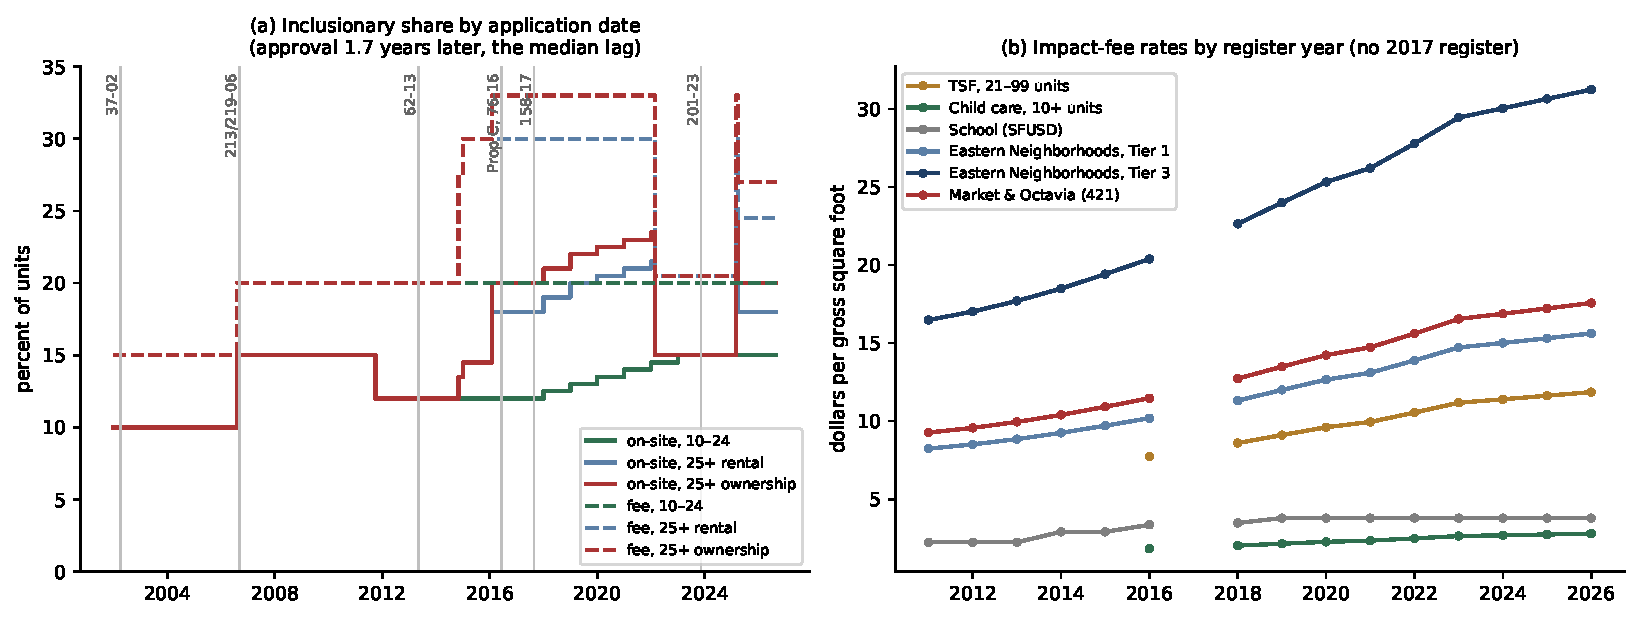
\includegraphics[width=\textwidth]{figures/fig_exaction_rates.pdf}
\caption{(a) The inclusionary share that vests, by application date, for a project approved
\exMedLag\ years later (the panel's median lag), from \texttt{inclusionary\_terms}; grey lines
mark the ordinances' effective dates. (b) The register rates of the main residential impact
fees; 2017 is a gap, not a line.}\label{fig:exrates}
\end{figure}

\section{Vesting: when each part is fixed}\label{sec:exvesting}

\extable{exvesting}

\paragraph{The share, 2002--2013: the first application.} Ordinance~219-06 says the prior
requirements apply to a project with a first site or building permit before its effective date;
Ordinance~62-13's own summary table keys the 2006 percentages to ``all projects that submitted
a first application on or after July 18, 2006'' and says the implementing ordinances prevail
over the table. The panel follows the table, and the conditions agree with it: of the
\exCrossSixN\ cases the schedule places under the 2006 version, \exCrossSix\% print a percentage
it assigns, and \exCrossTwo\% of the \exCrossTwoN\ under the 2002 version --- most of them filed
before July 2006 and approved years later at the 2002 rate. The same table dates the 2006
amendments' operation to \cl{inc2006_sep9}, which is also Legistar's passage date plus the
standard \cl{ord_effective_30days} (\exEffSixInferred).

\paragraph{The share, from 2016: the complete EEA.} The codified Sections~415.5 and 415.6 fix
the fee and the on-site percentage by ``the date that the project sponsor has submitted a
complete Environmental Evaluation application'', and the escalating on-site share is read at
that date. Two approval-date rules cut across it: the 2016 grandfathering lapses for a project
not approved by \cl{cod_4153_deadline}, and any vested requirement lapses without a site or
building permit within \cl{cod_4155_30months} of approval. The law is silent on one window: a
project filed after \cl{cod_4153_pre2016} and approved before \cl{inc2017_effective} must
comply with ``Sections 415.5, 415.6 and 415.7, as applicable''. The panel applies the version in
force at approval.

\paragraph{The fee in dollars: at payment.} The inclusionary fee is the vested share priced at
the rate in force when it is paid, at the first construction document; the fee is expressly
outside the 2023 approval-date freeze. Until the 2018 register the rate is an affordability gap
per unit by bedroom count; from 2019 it is a rate per gross square foot of residential floor
area times the share.

\paragraph{Impact fees: at payment, then at approval.} Every register from \exPaySentenceFirst\ to
\exPaySentenceLast\ says in its introduction that the adjusted rates ``apply to development impact fees paid on or after the effective date of any
such fee adjustments, regardless of the date of permit filing''; the sentence is gone from the register of
\exPaySentenceAbsent. Ordinance~193-23 (effective \cl{fee_193_effective}) fixed the types and
rates at Final Approval. From 2020 a housing project
with a complete SB~330 preliminary application is subject only to the standards in force when
it was filed, fees included, except for automatic index adjustments; the panel flags the
\exSbThreeThirty\ projects whose planning records mark SB~330 and does not re-date them.

\paragraph{Options, not assignments.} The 2023 pipeline relief is a modification the sponsor
requests (\exPipe\ projects are eligible); the 2023--26 rates apply only if the first
construction document follows approval within the deadline Section~415B sets. The panel carries the first beside the vested requirement and applies the
second where the permit dates show the condition met.

\section{The dollar rates}\label{sec:exrates}

\extable{exregisters}

Table~\ref{tab:exregisters} gives the residential rates. The area fees are charged only from
the date each took effect --- the Eastern Neighborhoods fee from \cl{area_en_start}, Market and
Octavia's from \cl{area_mo421_start}, Rincon Hill's from \cl{area_rh_start}, Central SoMa's from
\cl{area_cs_start} --- on the parcels today's fee-area layer places in them. The Transportation
Sustainability Fee applies to projects of \cl{tsf_threshold} or more units from \cl{tsf_created}, the
residential child-care fee from \cl{cc_created}. The jobs-housing linkage fee is a commercial
fee and is not charged to housing. For the 2017 rate year the panel uses the geometric mean of
the 2016 and 2018 rates and flags the projects priced with it.

\section{The panel}\label{sec:expanel}

The frame is every DBI new-construction permit (types 1 and 2) in the permits memo's
development-relevant universe that adds at least one unit and was filed from
\cl{inc2002_apply}, with a Commission case collapsed to its principal permit: \exProjects\
projects, \exLinked\ of them Commission-linked, \exBig\ of ten or more units. The
\exAlterations\ alterations that add units are set aside: after screening out revisions and
equipment permits they are still as often shoring and fire-main permits for a new building,
carrying its unit count, as they are conversions.

\extable{excoverage}

\paragraph{Dates.} The application date is the earliest environmental or project application
record of the case, else of any planning record that lists the permit, else the DBI filing
(\exDbiApp\% of projects, flagged). An environmental record's open date can precede its
acceptance as complete, so the EEA date is approximate. Approval is the Commission's approving
action, else DBI's approval or issuance; a project not yet approved is held to the version in
force at retrieval.

\paragraph{Floor area.} A project's residential floor area comes from its PRJ record where one
is linked and plausible for its unit count; otherwise it is the unit count times the median of
\exGpu\ gross square feet per unit across \exGpuN\ PRJ records of ten or more units
(interquartile range \exGpuLo--\exGpuHi). \exAssumedGfa\% of projects use the assumption. It is
an assumption, and it scales every per-square-foot fee.

\paragraph{Tenure, affordability, density bonus.} Tenure matters only above 25 units under
158-17 and for the Central SoMa fee. It is known for the projects MOHCD monitors and read from
descriptions for a few more; elsewhere the panel carries both and reports rental as the lower
bound. Projects that are 100\% affordable (Housing Production, MOHCD, or the description) are
outside the program and out of the distributions. The density-bonus flag is set by the pipeline
dataset's state density-bonus field or a mention in the permit, planning-record or minutes text;
the fee applies to bonus units, so the flag marks a project whose unit count includes them, and
its obligation --- like those of the UMU and SB~330 projects --- is marked uncertain in the panel
(\texttt{obligation\_uncertain}).

\paragraph{What is not modelled.} Area-specific inclusionary requirements --- Section~419 in the
UMU districts, special use districts, and the other areas Ordinance~201-23 lists --- replace the
citywide shares --- on \exUmu\ projects in UMU parcels alone; the panel keeps the citywide figures
and flags them. Credits for existing uses are not taken, so impact fees are gross. The TSF's own
grandfathering of earlier-filed projects is not modelled. The Van Ness and Market fee, charged
on floor area above a floor-area-ratio threshold, needs the FAR.

\section{The obligation}\label{sec:exobligation}

\extable{exobligation}

\begin{figure}[htbp]\centering
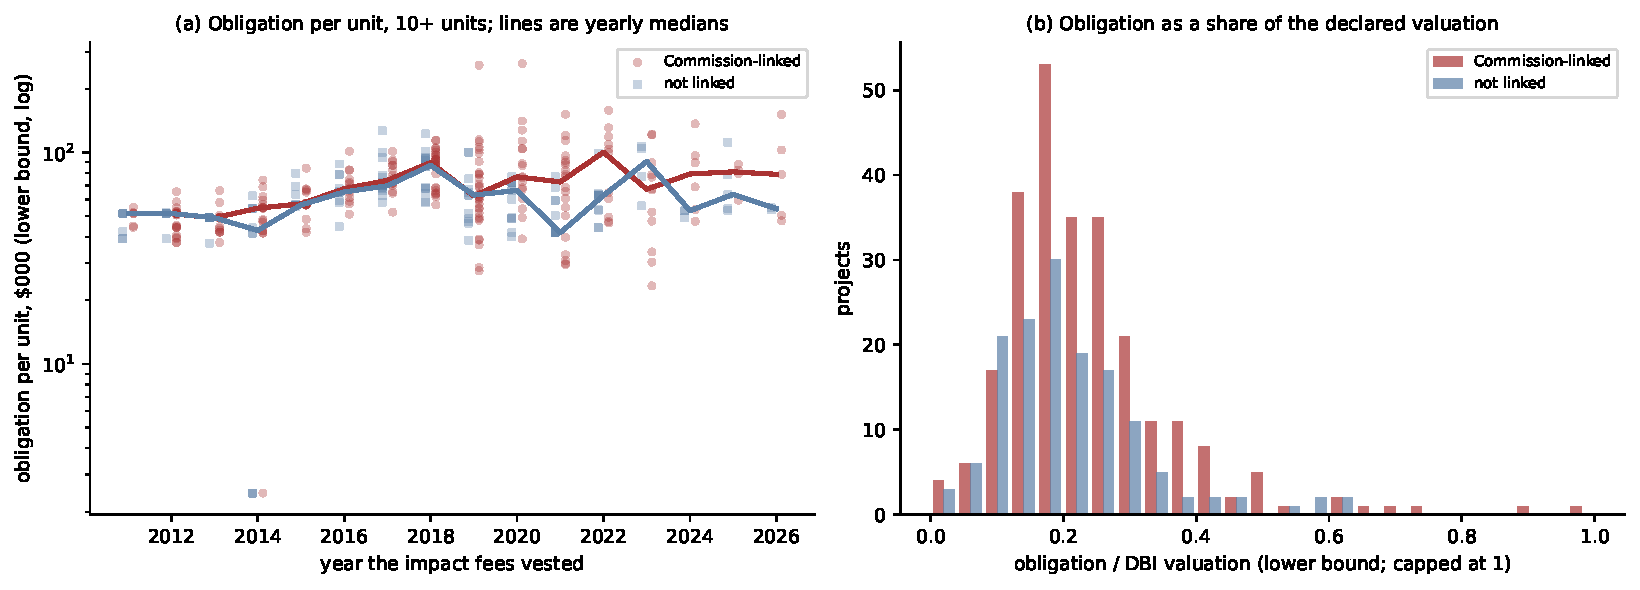
\includegraphics[width=\textwidth]{figures/fig_exaction_obligation.pdf}
\caption{(a) Obligation per unit for new buildings of ten or more units, by the year the
impact fees vested; points are projects, lines yearly medians. (b) The obligation as a share of
DBI's valuation. Lower bound (rental rates where tenure matters).}\label{fig:exobligation}
\end{figure}

Table~\ref{tab:exobligation} and Figure~\ref{fig:exobligation} give the distribution for new
buildings of ten or more units priced in full. The median per unit rose from \exPuMedA\ for fees
vested in 2011--15 to \exPuMedB\ in 2016--19 and was \exPuMedC\ and \exPuMedD\ after. The
inclusionary fee is most of it. Where tenure matters, the gap between the rental and ownership
figures is \exTenureGapMed\ per unit at the median.

Three cautions. The inclusionary requirement is priced at its fee, the price at which a sponsor
may buy out of building the units; a sponsor who builds on site chose to, so the fee bounds the
requirement's cost to that sponsor from above. The valuation is DBI's declared cost, which the
permits memo found understated, so the share of cost is an upper bound in the same direction.
And the impact fees are gross of credits.

\paragraph{Commission-linked and not.} The two groups owe similar amounts per unit
(\exPuMedLinked\ and \exPuMedNot\ at the median) and similar shares of valuation (\exShareMedLinked\%
and \exShareMedNot\%). Nothing here conditions on the project's size, place or year; the
comparison is a description.

\section{The schedule against the Commission's conditions}\label{sec:excross}

\extable{excross}

The conditions memo's numeric extraction reads the inclusionary percentage printed in a case's
conditions of approval. Where the case is in the panel the two can be compared
(Table~\ref{tab:excross}): \exCrossN\ cases (\exCrossRows\ condition rows), of which
\exCrossAgree\% print a percentage the schedule assigns the case, and \exCrossAgreeTwo\% of the
\exCrossNtwo\ outside the UMU districts and not wholly affordable.

The disagreements are informative. Under the grandfathered and lapsed versions agreement is low
(\exCrossGf\% of \exCrossGfN, \exCrossLapsed\% of \exCrossLapsedN): several projects approved
after \cl{cod_4153_deadline} print the grandfathered \cl{cod_4153_on135} or \cl{cod_4153_on145}
percent, which the text of Section~415.3 says they had lost, and some print the tier of the following year, which an EEA
accepted later than its record opened would explain. Some approvals in the months before
Ordinance~62-13 took effect already print its \cl{inc2013_table_onsite12} percent; Proposition~C of
\cl{propc2012}, which Ordinance~76-16 cites as codified in Charter Section~16.110, is a
candidate explanation whose terms were not read here. And the UMU and plan-area cases print
the area rates the panel does not model. The first two are the schedule's open questions; the
conditions are the Commission's statement of what it imposed, so they are evidence about how the
rules were applied, not errors to be corrected.

\section{Filing around rate changes}\label{sec:exbunching}

\begin{figure}[htbp]\centering
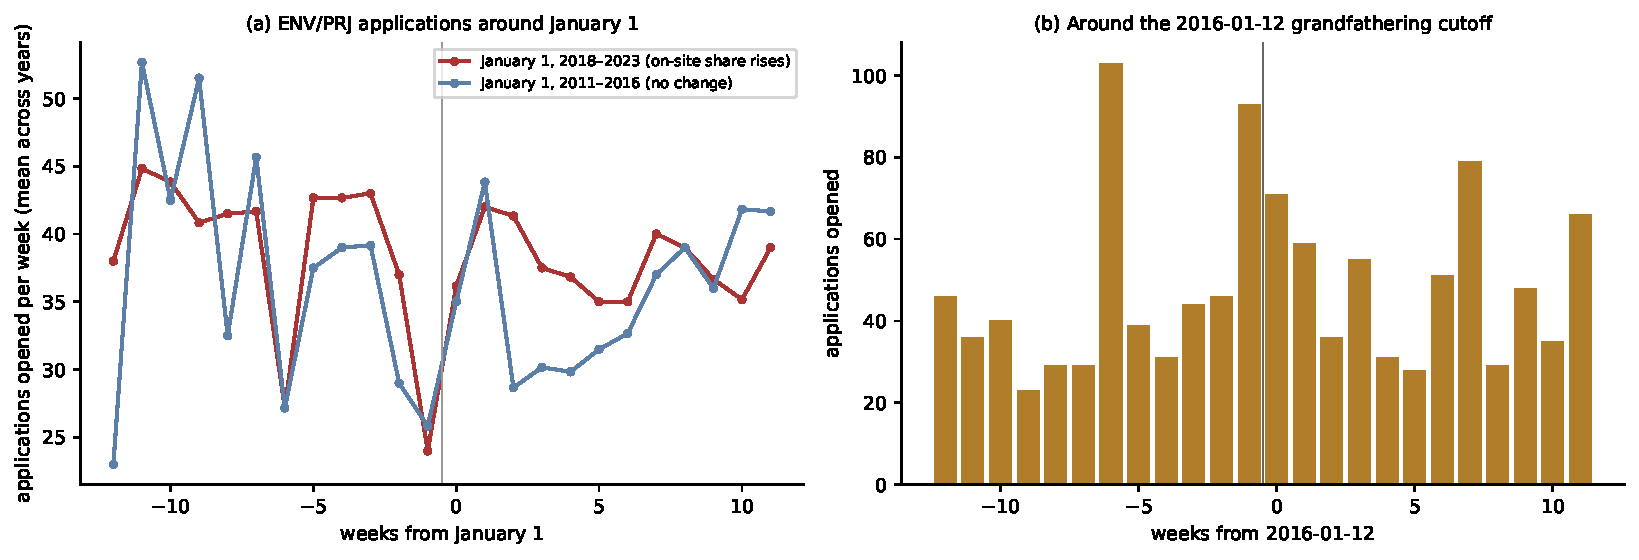
\includegraphics[width=\textwidth]{figures/fig_exaction_bunching.pdf}
\caption{(a) Environmental and project applications opened per week around January~1, averaged
over the years in which the on-site share rose on that date and over earlier years in which it
did not. (b) Around the 2016 grandfathering cutoff.}\label{fig:exbunching}
\end{figure}

From 2018 the on-site share rose each January~1 and was fixed by the EEA date, so a sponsor
ready to file had a reason to file in December. In the four weeks before those January~1st
\exBunchEscPre\ applications opened and in the four weeks after \exBunchEscPost\ (ratio
\exBunchEscRatio); in the same weeks of \exBunchNoPre\ against \exBunchNoPost\ in years without
an escalation (\exBunchNoRatio). Among PRJ records stating ten or more units the counts are
\exBunchTenPre\ and \exBunchTenPost. Around the 2016 cutoff, \exCutPre\ and \exCutPost. There is
no visible bunching.

This is a description. To be an estimate it needs the counterfactual weekly count --- the
holiday weeks are low every year, which is why the no-escalation years are shown --- a subset
of applications for which the escalation binds (projects of ten or more units, which the
records identify only from 2018), and the size of the step, which is \cl{cod_4156_esc_small} to \cl{cod_4156_esc_large1}
percentage points of the units. An EEA's open date is the record's creation, not its acceptance as complete, and the
two can differ by weeks.

\section{The ten-unit notch}\label{sec:exnotch}

\extable{exnotch}

\begin{figure}[htbp]\centering
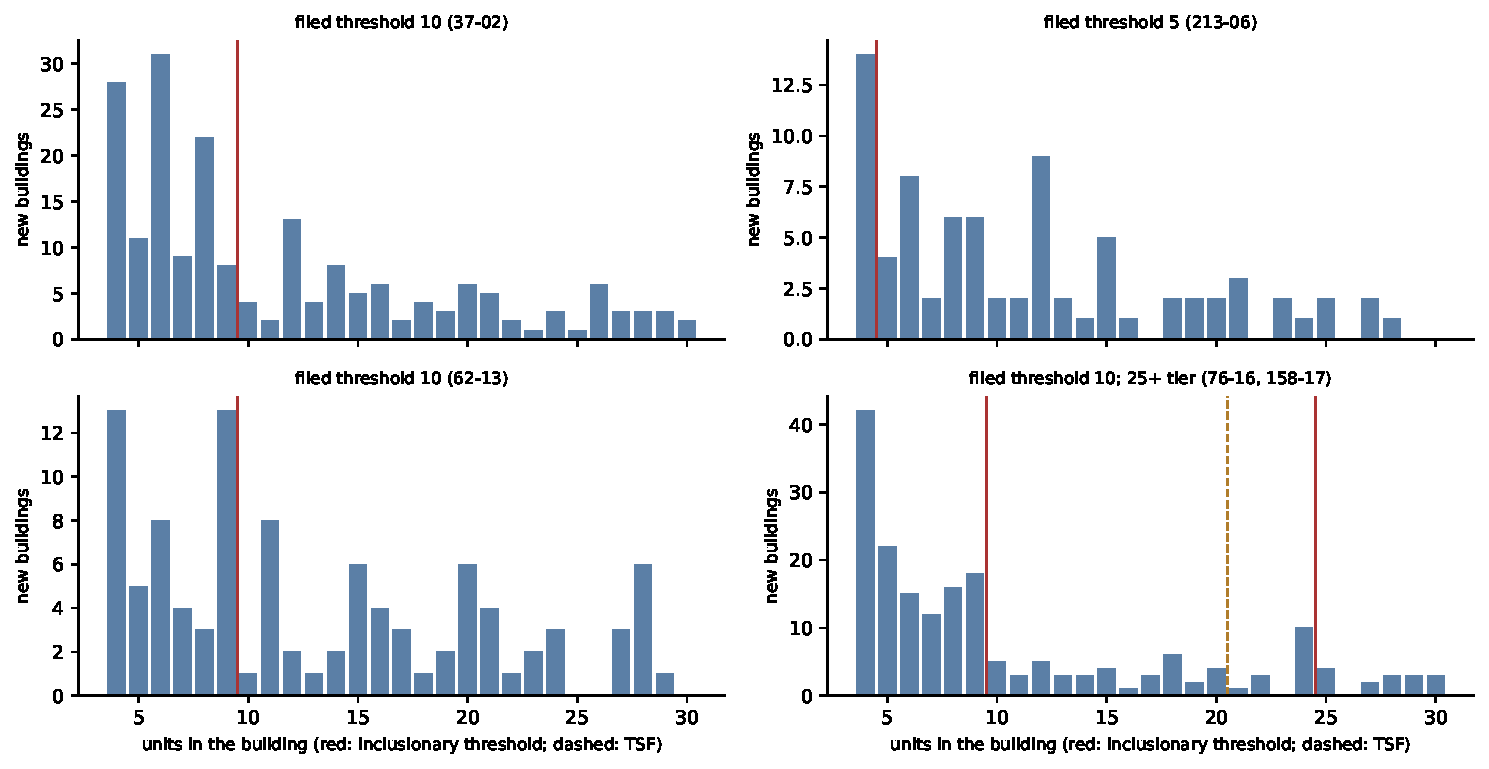
\includegraphics[width=\textwidth]{figures/fig_exaction_notch.pdf}
\caption{New buildings by unit count, by the version in force when they were filed; red lines
mark the inclusionary threshold (and from 2016 the 25-unit tier), the dashed line the TSF's.}
\label{fig:exnotch}
\end{figure}

A building of ten units owes the inclusionary requirement on all ten; one of nine owes nothing.
At \exStepYear\ rates the fee on a ten-unit building of median floor area is \exStepTen\
(\exStepTenPerUnit\ a unit). From 2016 the fee share rises at 25 units, which is worth
\exStepTwentyFive\ on a 25-unit rental building (\exStepTwentyFiveB\ under the 2023--26 rates),
and the TSF begins above 20 units (\exStepTsf\ on a 21-unit building).

In every version the count drops at the threshold (Table~\ref{tab:exnotch},
Figure~\ref{fig:exnotch}). Since 2016, \exNineA\ new buildings have nine units and \exTenA\ have
ten; \exTwentyFourA\ have 24 and \exTwentyFiveA\ have 25; \exTwentyA\ have 20 and \exTwentyOneA\
have 21. From 2006 to 2013, when the threshold was five, \exFourSix\ had four and \exFiveSix\
five, and nine and ten units were \exNineSix\ and \exTenSix. The counts are small and the
unit-count distribution falls with size anyway; what makes the pattern notable is that the drop
moves with the threshold. An estimate would compare the mass just below each threshold with a
smooth counterfactual fitted away from it, with the zoning envelope held fixed --- the parcel's
permitted density caps the unit count too, which is Part~5's panel.

\section{Established and not established}\label{sec:exest}

\paragraph{Established.}
\begin{enumerate}
\item The version chain of the inclusionary program from 2002 through the schedule operative
\cl{o201_operative}, every percentage and date quoted from the enacted ordinance, the codified
section or the Board's list, all \exClaimsVerified\ claims verified against their sources.
\item The residential impact-fee rates for every register year \exRegFirst--\exRegLast\ except
2017, quoted from the registers.
\item What vests when: the share by first application (2002--2013) and complete EEA (2016--);
the inclusionary fee in dollars at payment; impact fees at payment until \cl{fee_193_effective}
and at Final Approval since.
\item A new building of ten or more units priced in full owes a median \exPuMed\ per unit, most
of it the inclusionary fee, and Commission-linked projects owe about what others do.
\item New buildings are fewer just above each inclusionary threshold than just below it, and
the drop moves with the threshold.
\end{enumerate}

\paragraph{Not established.}
\begin{enumerate}
\item How the 2016 grandfathering deadline and the tier dates were applied: conditions of
projects approved after \cl{cod_4153_deadline} print grandfathered rates.
\item Which version bound a project filed between \cl{cod_4153_pre2016} and
\cl{inc2017_effective} and approved after the latter; the panel's rule (the version at
approval) is an assumption.
\item Area-specific requirements (UMU, special use districts) and the TSF's grandfathering;
credits for existing uses; the 2017 rates; dollar rates before \exRegFirst.
\item Floor area for the projects without a PRJ record, and tenure for most projects.
\item Any behavioural response: the bunching and notch sections are counts.
\end{enumerate}

\section{What remains}\label{sec:exremains}

\begin{itemize}
\item Source the area-specific requirements (Section~419's UMU tiers, Section~415.3(d) and the
special use districts) and model them.
\item Find the 2017 register and the pre-2011 registers (DBI posted them; the archive holds some
from 2011).
\item Resolve the grandfathering questions from MOHCD's published tables and the Planning
Department's inclusionary affidavits.
\item Take the TSF's grandfathering rules and existing-use credits from the codified sections.
\item Estimate the notch and the filing response, with the envelope from Part~5.
\end{itemize}

\section{Reproducing this}\label{sec:exrepro}

\begin{verbatim}
cd code/commission_minutes_processing
python build_exaction_panel.py fetch     # ordinance lists; every cited source
python build_exaction_panel.py claims    # write exaction_sources.csv
python build_exaction_panel.py probe     # verify every quotation
python build_exaction_panel.py build     # the project panel
python build_exaction_panel.py report    # tables, figures, macros
\end{verbatim}
Outputs: \texttt{\$MFHR\_DATA\_ROOT/external/exactions/} (\texttt{exaction\_projects.parquet},
\texttt{rate\_table.csv}, \texttt{parcel\_fee\_areas.parquet}, \texttt{claims\_checked.csv},
\texttt{crosscheck\_conditions.csv}, \texttt{bunching\_weeks.csv}, \texttt{notch\_counts.csv});
the sources and their text under \texttt{external/legal/}. The build reads the permit table and
linkage of \texttt{analyze\_permit\_content.py} and the planning records and fee-area join of
\texttt{acquire\_external\_data.py}.

\clearpage
\appendix
\section{The legal claims}\label{sec:exclaims}
\extable{exclaims}

\end{document}
